\documentclass{standalone}
\usepackage{tikz}
\usetikzlibrary{patterns, positioning}


\begin{document}
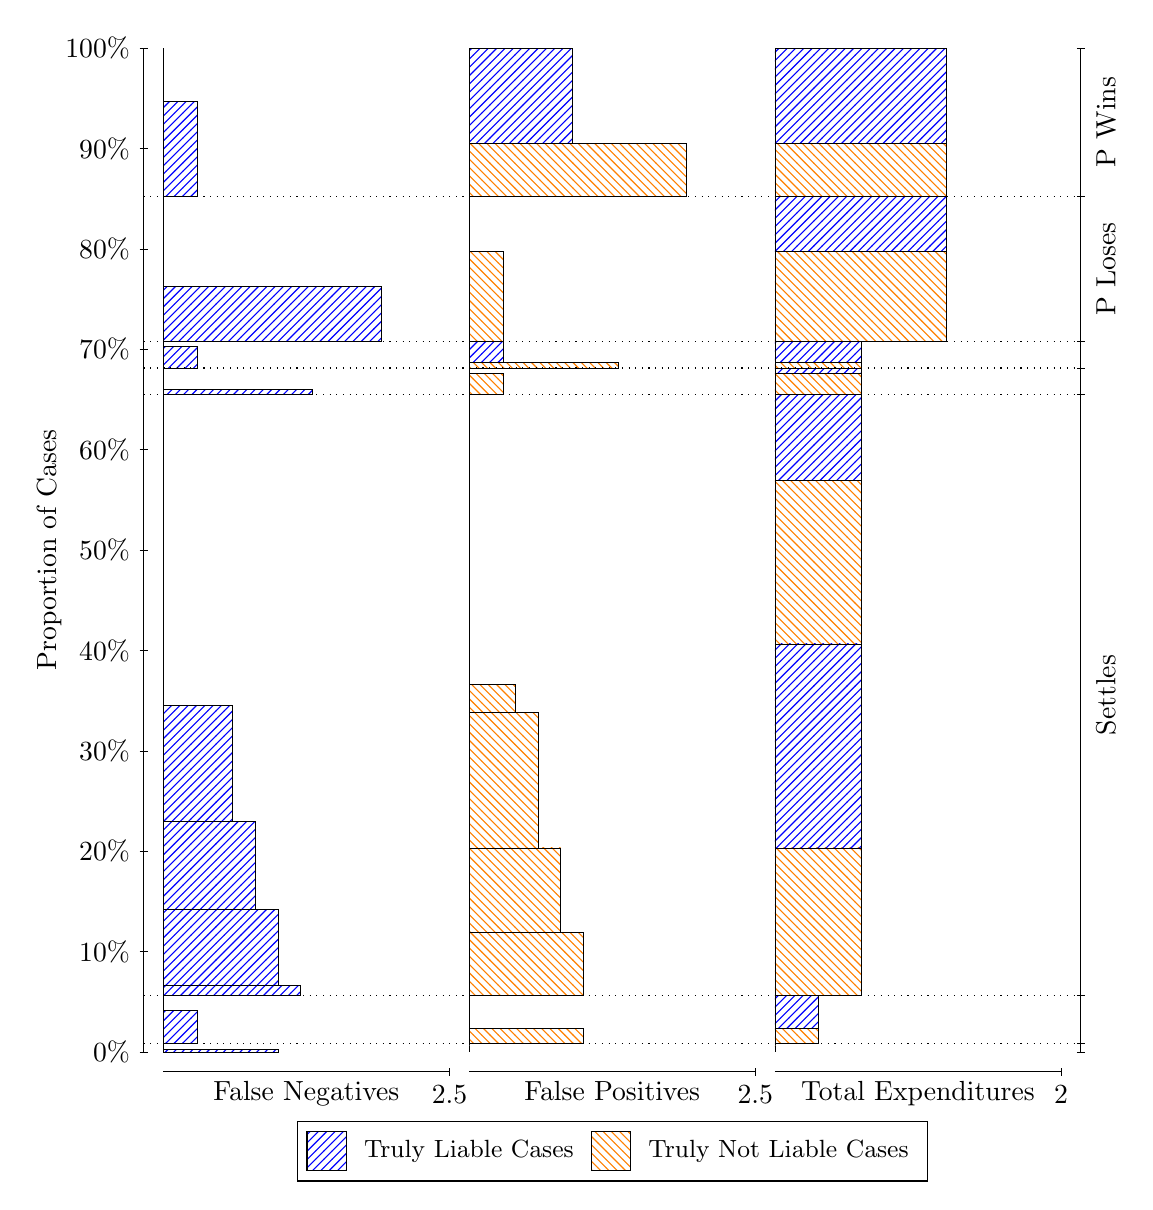
\begin{tikzpicture}
\draw[black, very thin] (1.5,1.75) -- (1.5,14.5);
\node[rotate=90, text=black, anchor=center] at (0.3, 8.125) {Proportion of Cases};
\draw[black, very thin] (1.45,1.75) -- (1.55,1.75);
\node[text=black, anchor=east] at (1.45, 1.75) {0\%};
\draw[black, very thin] (1.45,3.025) -- (1.55,3.025);
\node[text=black, anchor=east] at (1.45, 3.025) {10\%};
\draw[black, very thin] (1.45,4.3) -- (1.55,4.3);
\node[text=black, anchor=east] at (1.45, 4.3) {20\%};
\draw[black, very thin] (1.45,5.575) -- (1.55,5.575);
\node[text=black, anchor=east] at (1.45, 5.575) {30\%};
\draw[black, very thin] (1.45,6.85) -- (1.55,6.85);
\node[text=black, anchor=east] at (1.45, 6.85) {40\%};
\draw[black, very thin] (1.45,8.125) -- (1.55,8.125);
\node[text=black, anchor=east] at (1.45, 8.125) {50\%};
\draw[black, very thin] (1.45,9.4) -- (1.55,9.4);
\node[text=black, anchor=east] at (1.45, 9.4) {60\%};
\draw[black, very thin] (1.45,10.675) -- (1.55,10.675);
\node[text=black, anchor=east] at (1.45, 10.675) {70\%};
\draw[black, very thin] (1.45,11.95) -- (1.55,11.95);
\node[text=black, anchor=east] at (1.45, 11.95) {80\%};
\draw[black, very thin] (1.45,13.225) -- (1.55,13.225);
\node[text=black, anchor=east] at (1.45, 13.225) {90\%};
\draw[black, very thin] (1.45,14.5) -- (1.55,14.5);
\node[text=black, anchor=east] at (1.45, 14.5) {100\%};

\draw[black, very thin] (13.4,1.75) -- (13.4,14.5);
\draw[black, very thin] (13.35,1.75) -- (13.45,1.75);
\node[anchor=west] at (13.35, 1.75) {};
\draw[black, very thin] (13.35,1.8607) -- (13.45,1.8607);
\node[anchor=west] at (13.35, 1.8607) {};
\draw[black, very thin] (13.35,2.4662) -- (13.45,2.4662);
\node[anchor=west] at (13.35, 2.4662) {};
\draw[black, very thin] (13.35,10.098) -- (13.45,10.098);
\node[anchor=west] at (13.35, 10.098) {};
\draw[black, very thin] (13.35,10.436) -- (13.45,10.436);
\node[anchor=west] at (13.35, 10.436) {};
\draw[black, very thin] (13.35,10.775) -- (13.45,10.775);
\node[anchor=west] at (13.35, 10.775) {};
\draw[black, very thin] (13.35,12.615) -- (13.45,12.615);
\node[anchor=west] at (13.35, 12.615) {};
\draw[black, very thin] (13.35,14.5) -- (13.45,14.5);
\node[anchor=west] at (13.35, 14.5) {};

\draw[black, very thin, pattern color=blue, pattern=north east lines] (1.75,1.75) rectangle (3.2033,1.7804);
\draw[black, very thin, pattern color=orange, pattern=north west lines] (1.75,1.7804) rectangle (1.75,1.8607);
\draw[black, very thin, pattern color=blue, pattern=north east lines] (1.75,1.8607) rectangle (2.186,2.2775);
\draw[black, very thin, pattern color=orange, pattern=north west lines] (1.75,2.2775) rectangle (1.75,2.4662);
\draw[black, very thin, pattern color=blue, pattern=north east lines] (1.75,2.4662) rectangle (3.494,2.5995);
\draw[black, very thin, pattern color=blue, pattern=north east lines] (1.75,2.5995) rectangle (3.2033,3.5564);
\draw[black, very thin, pattern color=blue, pattern=north east lines] (1.75,3.5564) rectangle (2.9127,4.6798);
\draw[black, very thin, pattern color=blue, pattern=north east lines] (1.75,4.6798) rectangle (2.622,6.1496);
\draw[black, very thin, pattern color=orange, pattern=north west lines] (1.75,6.1496) rectangle (1.75,10.098);
\draw[black, very thin, pattern color=blue, pattern=north east lines] (1.75,10.098) rectangle (3.6393,10.164);
\draw[black, very thin, pattern color=orange, pattern=north west lines] (1.75,10.164) rectangle (1.75,10.436);
\draw[black, very thin, pattern color=blue, pattern=north east lines] (1.75,10.436) rectangle (2.186,10.709);
\draw[black, very thin, pattern color=orange, pattern=north west lines] (1.75,10.709) rectangle (1.75,10.775);
\draw[black, very thin, pattern color=blue, pattern=north east lines] (1.75,10.775) rectangle (4.5113,11.471);
\draw[black, very thin, pattern color=orange, pattern=north west lines] (1.75,11.471) rectangle (1.75,12.615);
\draw[black, very thin, pattern color=blue, pattern=north east lines] (1.75,12.615) rectangle (2.186,13.826);
\draw[black, very thin, pattern color=orange, pattern=north west lines] (1.75,13.826) rectangle (1.75,14.5);
\draw[black, very thin, pattern color=orange, pattern=north west lines] (5.6333,1.75) rectangle (5.6333,1.8303);
\draw[black, very thin, pattern color=blue, pattern=north east lines] (5.6333,1.8303) rectangle (5.6333,1.8607);
\draw[black, very thin, pattern color=orange, pattern=north west lines] (5.6333,1.8607) rectangle (7.0867,2.0493);
\draw[black, very thin, pattern color=blue, pattern=north east lines] (5.6333,2.0493) rectangle (5.6333,2.4662);
\draw[black, very thin, pattern color=orange, pattern=north west lines] (5.6333,2.4662) rectangle (7.0867,3.2684);
\draw[black, very thin, pattern color=orange, pattern=north west lines] (5.6333,3.2684) rectangle (6.796,4.3408);
\draw[black, very thin, pattern color=orange, pattern=north west lines] (5.6333,4.3408) rectangle (6.5053,6.0672);
\draw[black, very thin, pattern color=orange, pattern=north west lines] (5.6333,6.0672) rectangle (6.2147,6.4146);
\draw[black, very thin, pattern color=blue, pattern=north east lines] (5.6333,6.4146) rectangle (5.6333,10.098);
\draw[black, very thin, pattern color=orange, pattern=north west lines] (5.6333,10.098) rectangle (6.0693,10.37);
\draw[black, very thin, pattern color=blue, pattern=north east lines] (5.6333,10.37) rectangle (5.6333,10.436);
\draw[black, very thin, pattern color=orange, pattern=north west lines] (5.6333,10.436) rectangle (7.5227,10.503);
\draw[black, very thin, pattern color=blue, pattern=north east lines] (5.6333,10.503) rectangle (6.0693,10.775);
\draw[black, very thin, pattern color=orange, pattern=north west lines] (5.6333,10.775) rectangle (6.0693,11.92);
\draw[black, very thin, pattern color=blue, pattern=north east lines] (5.6333,11.92) rectangle (5.6333,12.615);
\draw[black, very thin, pattern color=orange, pattern=north west lines] (5.6333,12.615) rectangle (8.3947,13.29);
\draw[black, very thin, pattern color=blue, pattern=north east lines] (5.6333,13.29) rectangle (6.9413,14.5);
\draw[black, very thin, pattern color=orange, pattern=north west lines] (9.5167,1.75) rectangle (9.5167,1.8303);
\draw[black, very thin, pattern color=blue, pattern=north east lines] (9.5167,1.8303) rectangle (9.5167,1.8607);
\draw[black, very thin, pattern color=orange, pattern=north west lines] (9.5167,1.8607) rectangle (10.062,2.0493);
\draw[black, very thin, pattern color=blue, pattern=north east lines] (9.5167,2.0493) rectangle (10.062,2.4662);
\draw[black, very thin, pattern color=orange, pattern=north west lines] (9.5167,2.4662) rectangle (10.607,4.3408);
\draw[black, very thin, pattern color=blue, pattern=north east lines] (9.5167,4.3408) rectangle (10.607,6.934);
\draw[black, very thin, pattern color=orange, pattern=north west lines] (9.5167,6.934) rectangle (10.607,9.0078);
\draw[black, very thin, pattern color=blue, pattern=north east lines] (9.5167,9.0078) rectangle (10.607,10.098);
\draw[black, very thin, pattern color=orange, pattern=north west lines] (9.5167,10.098) rectangle (10.607,10.37);
\draw[black, very thin, pattern color=blue, pattern=north east lines] (9.5167,10.37) rectangle (10.607,10.436);
\draw[black, very thin, pattern color=orange, pattern=north west lines] (9.5167,10.436) rectangle (10.607,10.503);
\draw[black, very thin, pattern color=blue, pattern=north east lines] (9.5167,10.503) rectangle (10.607,10.775);
\draw[black, very thin, pattern color=orange, pattern=north west lines] (9.5167,10.775) rectangle (11.697,11.92);
\draw[black, very thin, pattern color=blue, pattern=north east lines] (9.5167,11.92) rectangle (11.697,12.615);
\draw[black, very thin, pattern color=orange, pattern=north west lines] (9.5167,12.615) rectangle (11.697,13.29);
\draw[black, very thin, pattern color=blue, pattern=north east lines] (9.5167,13.29) rectangle (11.697,14.5);
\draw[black, dotted] (1.5,1.8607) -- (13.4,1.8607);
\draw[black, dotted] (1.5,2.4662) -- (13.4,2.4662);
\draw[black, dotted] (1.5,10.098) -- (13.4,10.098);
\draw[black, dotted] (1.5,10.436) -- (13.4,10.436);
\draw[black, dotted] (1.5,10.775) -- (13.4,10.775);
\draw[black, dotted] (1.5,12.615) -- (13.4,12.615);
\draw[black, very thin] (1.75,1.5) -- (5.3833,1.5);
\node[text=black, anchor=north] at (3.5667, 1.5) {False Negatives};
\draw[black, very thin] (5.3833,1.45) -- (5.3833,1.55);
\node[text=black, anchor=north] at (5.3833, 1.45) {2.5};

\draw[black, very thin] (5.6333,1.5) -- (9.2667,1.5);
\node[text=black, anchor=north] at (7.45, 1.5) {False Positives};
\draw[black, very thin] (9.2667,1.45) -- (9.2667,1.55);
\node[text=black, anchor=north] at (9.2667, 1.45) {2.5};

\draw[black, very thin] (9.5167,1.5) -- (13.15,1.5);
\node[text=black, anchor=north] at (11.333, 1.5) {Total Expenditures};
\draw[black, very thin] (13.15,1.45) -- (13.15,1.55);
\node[text=black, anchor=north] at (13.15, 1.45) {2};



\node[text=black, centered, rotate=90] at (13.72, 6.2821) {Settles};


\node[text=black, centered, rotate=90] at (13.72, 11.695) {P Loses};
\node[text=black, centered, rotate=90] at (13.72, 13.558) {P Wins};

\draw (7.449999999999999,1.5) node[draw=none] (baseCoordinate) {};
\begin{scope}[align=center]
        \matrix[scale=0.5, draw=black, below=0.5cm of baseCoordinate, nodes={draw}, column sep=0.1cm]{
            \node[rectangle, draw, minimum width=0.5cm, minimum height=0.5cm, pattern color=blue, pattern=north east lines] {}; &
            \node[draw=none, font=\small, text=black] (B) {Truly Liable Cases}; &
            \node[rectangle, draw, minimum width=0.5cm, minimum height=0.5cm, pattern color=orange, pattern=north west lines] {}; &
            \node[draw=none, font=\small, text=black] (B) {Truly Not Liable Cases}; \\
            };
\end{scope}

\end{tikzpicture}
\end{document}